\documentclass[12pt]{article}
 
\usepackage[margin=1in]{geometry} 
\usepackage{amsmath,amsthm,amssymb}
\usepackage{graphicx} 
\newcommand{\N}{\mathbb{N}}
\newcommand{\Z}{\mathbb{Z}}
 
\newenvironment{problem}[2][Problem]{\begin{trivlist}
\item[\hskip \labelsep {\bfseries #1}\hskip \labelsep {\bfseries #2.}]}{\end{trivlist}}
\newenvironment{lemma}[2][Lemma]{\begin{trivlist}
\item[\hskip \labelsep {\bfseries #1}\hskip \labelsep {\bfseries #2.}]}{\end{trivlist}}
\newenvironment{exercise}[2][Exercise]{\begin{trivlist}
\item[\hskip \labelsep {\bfseries #1}\hskip \labelsep {\bfseries #2.}]}{\end{trivlist}}

\newenvironment{question}[2][Question]{\begin{trivlist}
\item[\hskip \labelsep {\bfseries #1}\hskip \labelsep {\bfseries #2.}]}{\end{trivlist}}
\newenvironment{corollary}[2][Corollary]{\begin{trivlist}
\item[\hskip \labelsep {\bfseries #1}\hskip \labelsep {\bfseries #2.}]}{\end{trivlist}}
 
\setlength{\parindent}{0pt}
\begin{document}
 
% --------------------------------------------------------------
%                         Start here
% --------------------------------------------------------------
 
\title{STA414 Assignment 3  }%replace X with the appropriate number
\author{Yuhao Zhao\\ %replace with your name
999878342} %if necessary, replace with your course title
 
\maketitle
 
\section{Fitting a Linear model}
estimated parameters :
\begin{verbatim}
Call:
lm(formula = Response ~ V1 + V2 + V3 + V4 + V5 + V6 + V7 + V8, 
    data = train)

Residuals:
     Min       1Q   Median       3Q      Max 
-1.40576 -0.31558 -0.03542  0.26756  1.95052 

Coefficients:
            Estimate Std. Error t value Pr(>|t|)    
(Intercept)  5.09323    0.44713  11.391  < 2e-16 ***
V1           0.21757    0.02145  10.142  < 2e-16 ***
V2           1.58882    0.71488   2.222  0.02718 *  
V3           2.56441    0.60984   4.205 3.68e-05 ***
V4           1.90180    0.44280   4.295 2.53e-05 ***
V5          -0.65827    0.23777  -2.769  0.00607 ** 
V6           0.30995    0.29234   1.060  0.29008    
V7           0.26580    0.05045   5.268 3.05e-07 ***
V8          -0.46711    0.11209  -4.167 4.30e-05 ***
---
Signif. codes:  0 ‘***’ 0.001 ‘**’ 0.01 ‘*’ 0.05 ‘.’ 0.1 ‘ ’ 1

Residual standard error: 0.5391 on 241 degrees of freedom
Multiple R-squared:  0.594,     Adjusted R-squared:  0.5805 
F-statistic: 44.07 on 8 and 241 DF,  p-value: < 2.2e-16

\end{verbatim}

From the summary table, we can see that the $R^2$ is about 0.6 which is somewhat not good enough. The variable V6 is not significant. So we can consider eliminate V6 in prediction.  \\

Using this simple linear model,we can predict of the data given by testing set. The mean square error is 0.2944


\section{Fitting a Gaussian process models }

i) For the model with linear covariance: the Mean Square Error is 0.443493 \\

ii) For the model with hyperparameters $\gamma, \rho $\\

a) the cross validation result (the MSE vs parameters):\\
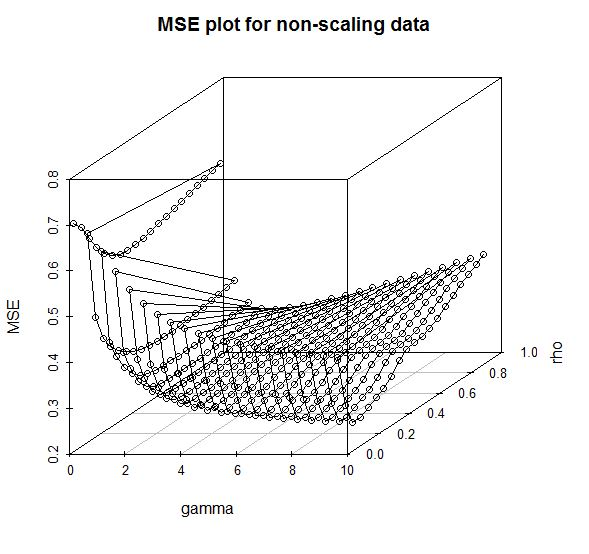
\includegraphics[width=3in]{1}	
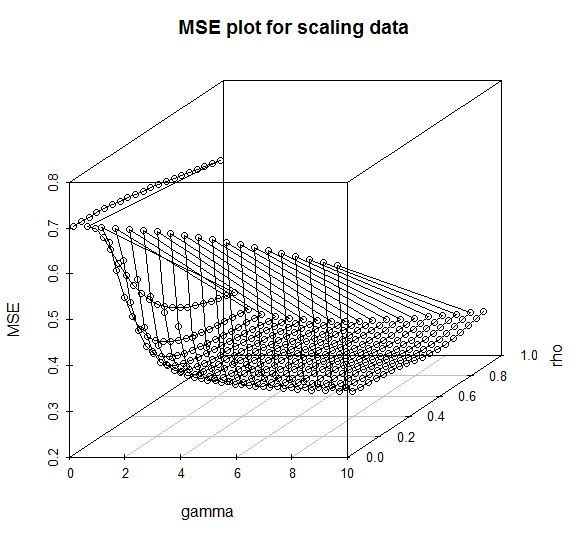
\includegraphics[width=3in]{2}

The optimal solution for hyperparameters to minimize MSE are:\\

 $\gamma = 9.6, \rho = 0.16 $ for original data\\
 $\gamma = 4.6, \rho = 0.96 $ for scaling data\\

The mean squared error for testing is:\\

 For the original data, Mean testing error  = 0.2935\\
 For the scaling data, Mean testing error  = 0.2406\\

\cleardoublepage 

\section{Summary}
\begin{verbatim}
-----------------------------------------------------------------
| Method |   Linear   |   GP with   |  GP with hyperparameters  |
|        | Regression | linear cov  |  original   |  scaling    |
-----------------------------------------------------------------
|  MSE   |   0.2944   |   0.4435    |   0.2935    |   0.2406    |
|  Time  |     5s     |    45s      |   30mins    |   30mins    |
-----------------------------------------------------------------
\end{verbatim}

The Gaussian Process with linear covariance works the worst, because the parameter isn't well chosen to minimize the mean square error. The Gaussian process regression for original dataset works similiar to the simple linear regression, but it takes much longer time to find the optimal hyperperameters. Gaussian process model after rescaling works slightly better but it still requires about 30 mins to find hyperperameters.
\cleardoublepage 

\section{code}
\begin{verbatim}
% % %covariance function1 
function [ out ] = K1(i,j )
out = 100^2*dot(i,j);
end.

% % %covariance function2 
function [ out] = K2(gamma,rho,x,y)
out = 100^2+gamma^2*exp(-rho^2*(sum((x-y).^2)));
end

% % %function to get the desired dataset for cross validation
function [out1_x out2_x out1_y out2_y] = split(trainx,trainy, i )
out2_x = trainx;
out1_x = trainx(((i-1)*25+1):(i*25),:);
out2_x(((i-1)*25+1):(i*25),:) = [];
out2_y = trainy;
out1_y = trainy(((i-1)*25+1):(i*25));
out2_y(((i-1)*25+1):(i*25)) = [];
end

% % % function that return sum MSEs for cross validation given parameters
function [ out ] = estimate_(gamma,rho,trainx,trainy)
MSE = zeros(1,10);
for k = 1:10
    [x_test,x_train,y_test,y_train] = split(trainx,trainy,k);
    C = zeros(225,225);
    for i=1:225
        for j = i:225
        C(i,j) = K2(gamma,rho,x_train(i,:),x_train(j,:)) ;
        C(j,i) = C(i,j);
        end   
    end
    C = C + eye(225);
    
    predict = zeros(1,25);
    for i = 1:25
        t = zeros(1,225);
        for j = 1:225
            t(j) = K2(gamma,rho,x_train(j,:),x_test(i,:)) ;
        end
         predict(i) = t*pinv(C)*y_train;
    end
    
    MSE(k) = sum((transpose(y_test) - predict).^2);
      
end
out = sum(MSE);
end

% % %Main function
[trainx] = textread('train1x.txt','');
[trainy] = textread('train1y.txt','');
[testx] = textread('testx.txt','');
[testy] = textread('testy.txt','');

%%%fitting a Gausian process model with linear covariance 
C = zeros(250,250);
for i=1:250
    for j = 1:250
    C(i,j) = K1(trainx(i,:),trainx(j,:)) ;
    end   
end

C = C+eye(250);

predict = zeros(1,2500);
for i = 1:length(testy)
    t = zeros(1,250);
    for j = 1:250
    t(j) = K1(trainx(j,:),testx(i,:)) ;
    end
    predict(i) = t*(C\trainy);
end

MSE_2  = sum((transpose(testy) - predict).^2)/2500;

%%% fitting Gaussian provess model for non-scaling data
out = zeros(3,400);
count = 1;
for gamma = 0.1:0.5:10
    for rho = 0.01:0.05:1
        out(:,count) = [estimate_(gamma,rho,trainx,trainy);gamma;rho];
        count = count+1;
        [count, out(1,count-1),out(2,count-1),out(3,count-1)]
    end


end


dlmwrite('out1.txt',out,'\t')

index = find(out(1,:) ==min(out(1,:)));
gamma = out(2,index);
rho = out(3,index);

C = zeros(250,250);
for i=1:250
    for j = 1:250
    C(i,j) = K2(gamma,rho,trainx(i,:),trainx(j,:)) ;
    end   
end
 C = C + eye(250);
 

predict = zeros(1,2500);
for i = 1:length(testy)
    t = zeros(1,250);
    for j = 1:250
    t(j) = K2(gamma,rho,trainx(j,:),testx(i,:)) ;
    end
    predict(i) = t*(C\trainy);
end

MSE_3_a = sum((transpose(testy) - predict).^2)/2500;

%%% fitting Gaussian provess model for scaling data

trainx_ = trainx;
testx_ = testx;
trainx_(:,1) = trainx(:,1)/10 ;
trainx_(:,7) = trainx(:,7)/10;
testx_(:,1) = testx(:,1)/10 ;
testx_(:,7) = testx(:,7)/10;

out_2 = zeros(3,400);
count = 1;
for gamma = 0.1:0.5:10
    for rho = 0.01:0.05:1
        out_2(:,count) = [estimate_(gamma,rho,trainx_,trainy);gamma;rho];
        count = count+1;
        [count, out_2(1,count-1),out_2(2,count-1),out_2(3,count-1)]
    end

end
index = find(out_2(1,:) ==min(out_2(1,:)));
gamma = 4.6;
rho = 0.96;

C = zeros(250,250);
for i=1:250
    for j = 1:250
    C(i,j) = K2(gamma,rho,trainx_(i,:),trainx_(j,:)) ;
    end   
end
 C = C + eye(250);
 

predict_2 = zeros(1,2500);
for i = 1:length(testy)
    t = zeros(1,250);
    for j = 1:250
    t(j) = K2(gamma,rho,trainx_(j,:),testx_(i,:)) ;
    end
    predict_2(i) = t*(C\trainy);
end

MSE_3_b = sum((transpose(testy) - predict_2).^2)/2500;


\end{verbatim}


\end{document}

